\section{Implementing CustomGraphSearch}
 %\setcounter{page}{2}
 %\addtocounter{section}{1}
 \thispagestyle{empty}
\subsection{Aim}

This first lab session explores the concept of intelligents agents. The agent is a
Vacuum cleaner evolving in a simple grid. Each square of that grid is either clean
or filled with dirt. The agent can only perform basic actions :
move forward, turn right, turn left and suck.
The purpose of this lab is to write an algorithm to automate the cleaning process.
No supposition regarding the world dimension or the dirt position can be made.
The vacuum cleaner has to be completly autonomous.
\subsection{Strategy}
Given that this first assignement does not imply obstacle avoidance, it is possible
to implement an easy 3-step strategy :
The variable \textit{uMovement} is used as a conditional counter in this sequence.
\newpage This sequence is composed of three movements :
\begin{itemize}
  \item Turning 90° in the given direction (\textit{uMovement equal to 0})
  \item Moving forward, down to the next grid line (\textit{uMovement equal to 1})
  \item Turning again in the same direction (\textit{uMovement equal to 0 again})
\end{itemize}

\subsection{Possible improvement}

Given that the java GUI give us the ability to add obstacles in the grid,
an interesting improvement would be to implement search algorithms in order to
find the best path while avoiding collision.

\begin{figure}[h]
    \centering
    %  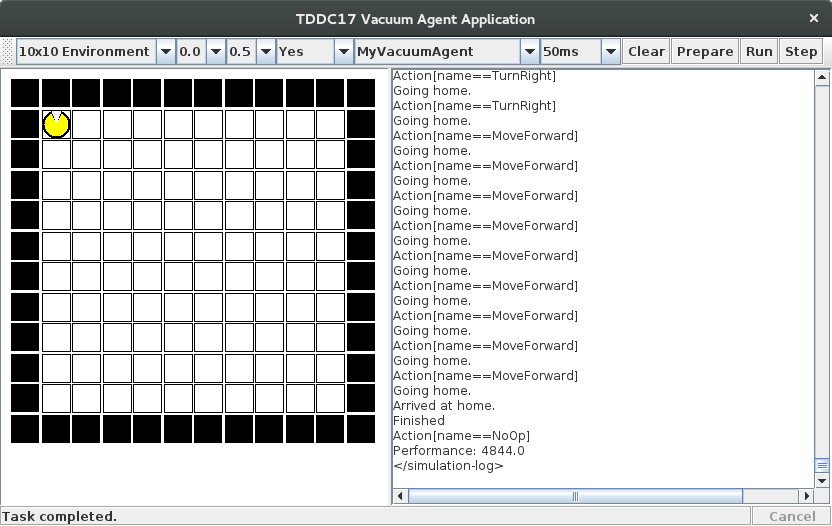
\includegraphics[width=0.83\linewidth]{./images/lab_1.png}
    \caption{Screenshot\label{Vacuum cleaner}}
\end{figure}

\newpage
\thispagestyle{empty}
\section{Theory}

\paragraph{Question 1}
\paragraph{Question 2}
\paragraph{Question 3}
\paragraph{Question 4}
\paragraph{Question 5}
\paragraph{Question 6}
\paragraph{Question 7}
